\chapter{Einleitung}
Inhalt dieses Projektes ist die Erstellung eines \acs{SDR}, wobei ein \acs{FPGA} als Plattform dienen soll. 
Der \acs{FPGA}-Logikteil soll weiterhin von einem Rechenkern, für die weitere Datenverarbeitung, unterstützt werden.

Da es sich um ein Lernprojekt handele, sollte der Fokus, bei der Erstellung der \acs{FPGA}-Schaltung, auf der selbständigen Erstellung aller Signal verarbeitenden Blöcke liegen.
Komplexe Blöcke welche für die Kommunikation mit dem Rechensystem benötigt wurden \textit{(z.B. AXI-Infrastruktur)} wurden aus Zeitgründen nicht selbst erstellt, sondern vorhandene
IP-Kerne des \acs{FPGA}-Herstellers verwendet.

\section{Anforderungen}
Zu beginn des Projektes wurde mit der Festlegung der Anforderungen an des Gesamtsystem begonnen. Folgend konnten die notwendigen Hardware- und Logikkomponenten richtig ausgelegt werden.

Dabei wurden die folgende Anforderungen an das System definiert:
\begin{enumerate}
	\item \textbf{Unterstützung der Verwendung eines extern \acs{ADC}}
	\begin{enumerate}[label*=\arabic*.]
		\item Abtastfrequenz von mindestens \qty{100}{M\hertz} [$f_{ADC} \ge \qty{100}{M\hertz}$].
		\item Datenbreite soll mindestens \qty{12}{bit} betragen [$w_{adc} \ge 12$]
		\item Externer Antialias Filter notwendig, Abtastung in der ersten Nyquist-Zone.
	\end{enumerate}

	\item \textbf{Digitale Abwärtsmischung in das Basisband}
	\begin{enumerate}[label*=\arabic*.]
		\item Eingangssignal im Frequenzbereich \qty{1}{M\hertz} bis \qty{20}{M\hertz}. [$f_s \in [\qty{1}{M\hertz};\qty{20}{M\hertz}]$]
		\item Interner \acl{NCO}, wobei die Frequenz innerhalb des Frequenzbereichs konfigurierbar sein soll
		\item Interner, komplexer Mischer mit $\qty{16}{bit}$-Breitem $I/Q$ Signal am Ausgang
		\item Dezimierungsfilter mit, zum Synthesezeitpunkt einstellbaren, variablen Dezimierungsverhältnis
		\item Eine interne \acs{FPGA}-Taktrate von $f_{clk} \ge \qty{200}{M\hertz}$ soll unterstützt werden.
	\end{enumerate}

	\item \textbf{Carrier-Tracking für \acs{BPSK} und \acs{QPSK} Signale}
	\begin{enumerate}[label*=\arabic*.]
		\item Interner Phasen-Komparator mit folgendem Regler zur Konditionierung des lokalen Oszillators.
		\item Modulation (\acs{BPSK}/\acs{QPSK}) soll zur Laufzeit wechselbar sein.
		\item Als Regler soll ein $PID$-Regler mit, zur Laufzeit einstellbaren Koeffizienten, sein.
		\item Das Carrier-Tracking soll Abschaltbar sein und nur aktiv sein wenn das Eingangssignal eine gewisse Amplitude aufweist.
	\end{enumerate}

	\item \textbf{Kommunikation mit dem Rechenkern}
	\begin{enumerate}[label*=\arabic*.]
		\item Ein Rechenkern soll die \acs{FPGA}-Schaltung verwalten und die weitere Verarbeitung der Nutzdaten übernehmen.
		\item Die Steuerung der einzelnen Module soll der Rechenkern über eine \acs{AXI}-Lite Registerbank vornehmen können.
		\item Die gemischten und dezimierten Nutzdaten sollen via \acl{DMA}-Controller dem Rechenkern zur Verfügung gestellt werden.
	\end{enumerate}
\end{enumerate}


\section{Auswahl der Hardware-Komponenten}
Nach Festlegung der Anforderungen wurde die für die Umsetzung notwendige Hardware ausgewählt.

Aufgrund der Anforderung $4.1$ sowie dem Fokus der Vorlesung, FPGA-Logik in \acs{CPU}-Rechensysteme zu integrieren, 
ist es notwendig einen \acs{FPGA} mit eingeschlossenen \acs{CPU}-Kernen auszuwählen.

Die Wahl fiel hier aus Kosten- und da Know-How-Gründen sowie aufgrund der bereits Vorhandenen Tool-Umgebung, auf die Zynq-7000 \acs{APSoC} Serie des Herstellers Xilinx.
Es handelt sich hierbei um eine \acs{FPGA}-Fabric der Xilinx 7-Series \textit{(PL,Programmable-Logic)} mit angeschlossenem Dual-Core ARM Cortex-A9 \textit{(PS,Processing-System)}
als Rechenkern.

\begin{figure}[h]
	\centering
	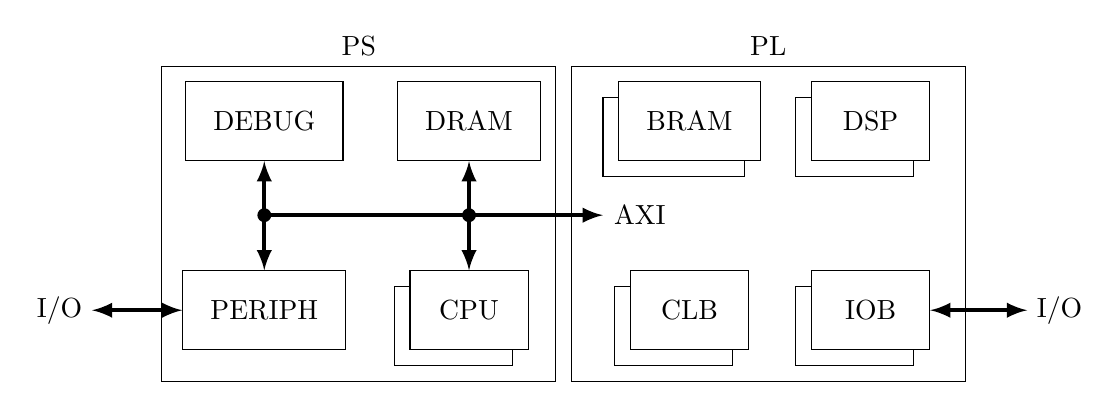
\begin{tikzpicture}
		\def\wrow{10.9}
		\def\xrow{8.5}
		\def\yrow{6.2}
		\def\zrow{7.2}
		\def\arow{2}
		\def\brow{3.4} 	
		\def\crow{0.8}
		\def\drow{-1.8}
	
		\tikzset{
			basic/.style={rectangle,draw=black, top color=white,text centered},
			bignode/.style={basic, inner sep=1em,minimum width=5cm, minimum height=4.0cm},	
			smallnode/.style={basic, inner sep=1em,minimum width=1.5cm, minimum height=1cm},
			branch/.style={fill,circle,minimum size=5pt,inner sep=0pt,outer sep=-1pt},
			sarrow/.style={->, >={latex}, line width=1.5pt},
    		carrow/.style={<->, >={latex}, dashed}
 		}
 		
 		\node[bignode, label=above:PS] (PS) at (\arow,2) {};
 		\node[smallnode] (PS_CPU0)   at (\brow-0.2,0.7) {CPU};
 		\node[smallnode] (PS_CPU1)   at (\brow,0.9) {CPU};
 		\node[smallnode] (PS_DRAM)   at (\brow,3.3) {DRAM};
 		\node[smallnode] (PS_DEBUG)  at (\crow,3.3) {DEBUG};
 		\node[smallnode] (PS_PERIPH) at (\crow,0.9) {PERIPH};

		\node[bignode, label=above:PL] (PL) at (\zrow,2){};		
 		\node[smallnode] (PL_CBL0)   at (\yrow-0.2,0.7) {CLB};
 		\node[smallnode] (PS_CBL1)   at (\yrow,0.9) {CLB}; 
 		
 		\node[smallnode] (PL_BRAM0)   at (\yrow-0.2,3.1) {BRAM};
 		\node[smallnode] (PS_BRAM1)   at (\yrow,3.3) {BRAM}; 
 		
 		\node[smallnode] (PL_DSP0)   at (\xrow-0.2,3.1) {DSP};
 		\node[smallnode] (PS_DSP1)   at (\xrow,3.3) {DSP}; 		
 		
 		\node[smallnode] (PL_IOB0)   at (\xrow-0.2,0.7) {IOB}; 	
 		\node[smallnode] (PL_IOB1)   at (\xrow,0.9) {IOB}; 		
 		
 		\node (PS_IO) at (\drow,0.9) {I/O};
 		\node (PL_IO) at (\wrow,0.9) {I/O};
 		
 		\draw[sarrow, <->] (PS_IO) -- (PS_PERIPH.west);
 		\draw[sarrow, <->] (PS_PERIPH.north) -- ++(0,0.7) node[branch](psb0){} -- (PS_DEBUG.south);
 		\draw[sarrow, <->] (PS_CPU1.north) -- ++(0,0.7) node[branch](psb1){} -- (PS_DRAM.south);
		\draw[sarrow, ->] (psb0) -- (psb1) -- ++(1.7,0) node[anchor=west]{AXI}; 		
		
		\draw[sarrow, <->] (PL_IOB1) -- (PL_IO);
 		
	\end{tikzpicture}
	\caption{Struktur des verwendeten Zynq-7000 \acs{FPGA}}
\end{figure}

Die in der \acs{FPGA}-Fabric (PL-Teil) vorhandenen Logic-Resourcen \textit{(\acs{BRAM},\acs{CLB},\acs{IOB}, \acs{DSP}-Slices)} werden gemäß des während der Implementierung erstellen
\acs{FPGA}-Designs verdrahtet und am Ende durch einen \acs{AXI}-Bus mit dem Rechensysteme (PS-Teil) verbunden. 

Da der \acs{FPGA} mit \acs{ADC} Modul selbst beschafft und bezahlt wird war hier vor allem der Preis ausschlaggebend.
Die Wahl fiel hier auf ein Eclypse Z7 Board der Firma Digilent.

\begin{figure}[h]
	\centering
	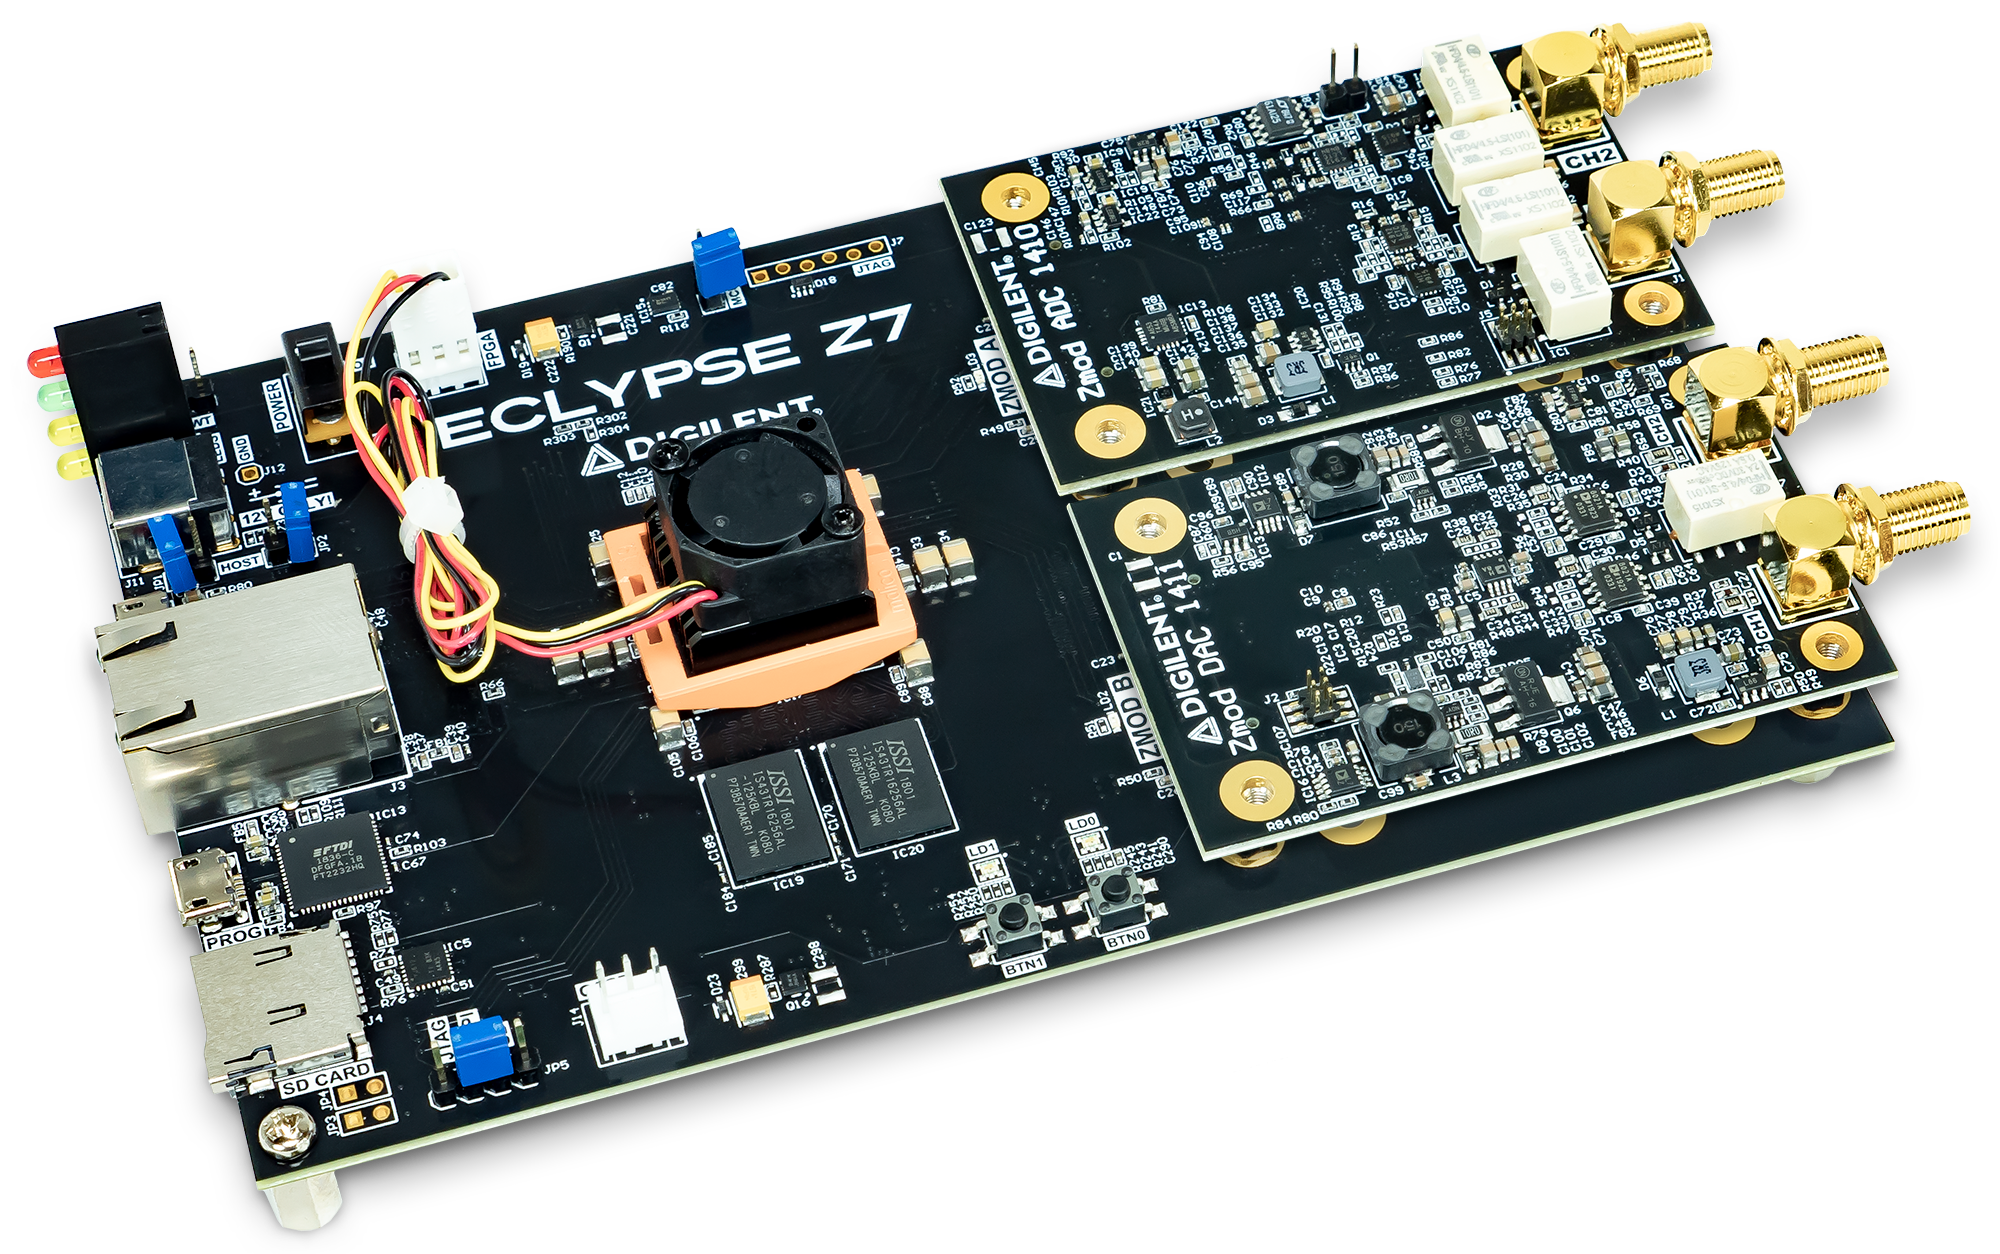
\includegraphics[width=15cm]{Eclipse-Z7}
	\caption{Bild des Eclypse-Z7 mit ADC und DAC} \faCopyright Digilent Inc. \cite{DIG_EZ7_REF}
\end{figure}

Hauptgrund für die Auswahl dieses Boards war der, im Vergleich zu anderen FPGA Mezzanine Card (FMC) basierten Boards, relativ günstige Preis, sowie das Vorhandensein von
vielen IP-Cores der Firma Digilent welche die Ansteuerung der einzelnen Hardware-Komponenten vereinfachen. Zusätzlich hilfreich war der große Umfang von verfügbaren Referenzmaterialien.

Der von dem Board verwendete \acs{ADC} \textit{(ZModScope 1410-105, AD9648BCPZ-105)} erfüllt alle gestellten Anforderungen.\cite{DIG_EZ7_ADC_REF}

Bei dem verwendeten \acs{FPGA} handelt es sich um einen XC7Z020-1CLG484C mit Dual-Core Cortex-A9 Prozessor mit \qty{666}{M\hertz}, sowie \qty{1}{GiB} externem DDR3-DRAM\cite{DIG_EZ7_REF}

Ein DAC wäre ebenfalls vorhanden, wird jedoch nicht genutzt.

